\section{Cross-field demonstration: cancer mutation-signature tasks}\label{sec:7}

The claim that $Q(s,a)$ is modality-agnostic is structural. The four primary modalities (text, vision, audio, world) test it within sequence-shaped or grid-shaped data. A harder test is whether the same block transfers to a domain where the input is not a sequence in the linguistic or sensory sense at all. We run four cross-field demonstrations: signature decomposition, pan-cancer classification, drug-response regression, and 5-year survival prediction. Each phase uses the identical SAVO block class; only the I/O layers and the output head differ.

\subsection*{Phase 1: COSMIC SBS96 signature decomposition}

Given $v \in \Delta^{96}$ (a tumor's SBS96 context distribution), recover $c \in \Delta^{K}$, the mixture over $K$=79 COSMIC reference signatures \cite{ref28} such that $v \approx Sc$. The domain baseline is non-negative least squares (NNLS) applied directly to the fixed signature dictionary $S \in \mathbb{R}^{96\times 79}$ --- the arithmetic that SigProfilerAssignment \cite{ref29} performs internally. On synthetic mixtures (50,000 train / 2,000 val) NNLS reaches mean cosine similarity 0.987 and top-1 exact-signature recovery 0.961.

\paragraph{Architecture.} A 14.86M-parameter SAVO stack ($H$=384, $r$=48, 6 encoder + 4 transition layers, $h$=6, MH-QVC) with a context-embedding front-end ($\log(1+\text{count})\cdot W_{\text{count}} + \text{ctx\_embed}$) and a softmax head over $K$ signatures (Fig.~\ref{fig:10}). Cross-entropy with a soft target plus an auxiliary MSE term enforcing $S\hat{c} \approx v$.

\begin{figure}[tbp]
  \centering
  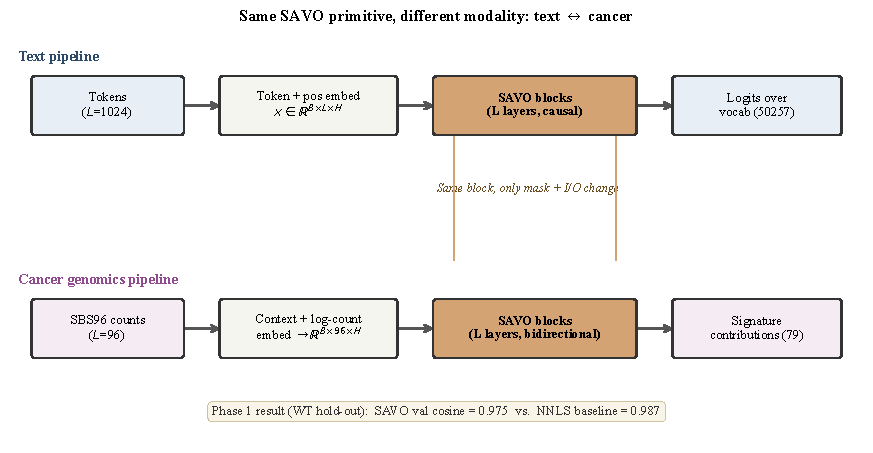
\includegraphics[width=.929\linewidth]{figs/fig10.pdf}
  \caption{\textbf{Same SAVO primitive, different modality.} Top: text pipeline with token + positional embeddings and 50,257-vocab logits. Bottom: cancer-genomics pipeline with mutation-context + log-count embeddings and a softmax over 79 COSMIC SBS signatures. Only the I/O layers and the causal mask differ; the SAVO block is the same class.}
  \label{fig:10}
\end{figure}

\paragraph{Result.} Trained from random initialization for 15,000 steps (batch 64, cosine-annealed LR, Muon for 2D weights and AdamW for biases/embeddings, bf16 AMP), the SAVO cancer model reaches held-out cosine similarity 0.975 --- 0.012 cosine below NNLS. Top-1 exact-signature recovery is 0.878 (NNLS 0.961); reconstruction MSE is $2\times 10^{-5}$. SAVO 0.975 vs NNLS 0.987: NNLS is the higher number, which is expected --- signature decomposition with $S$ known is a convex non-negative least-squares problem and NNLS is near-optimal on it. The architectural claim is invariance of the routing primitive across domains, not domain superiority.

\begin{figure}[tbp]
  \centering
  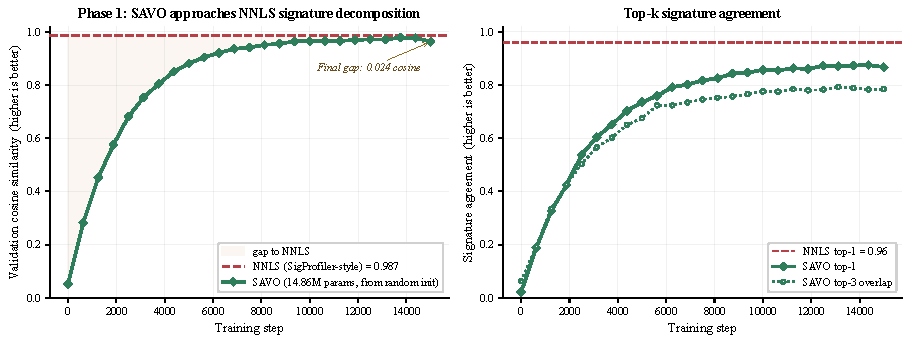
\includegraphics[width=.969\linewidth]{figs/fig11.pdf}
  \caption{\textbf{Phase 1 convergence.} Left: validation cosine similarity over training steps (green) vs.\ the NNLS baseline (red dashed). Shaded area indicates the residual gap. Right: top-1 and top-3 signature agreement.}
  \label{fig:11}
\end{figure}

SAVO does not beat NNLS on its home turf, and we did not expect it to: signature decomposition is a convex non-negative least-squares problem for which NNLS is near-optimal when $S$ is known. The architectural claim is invariance of the primitive across domains.

\subsection*{Phase 2: pan-cancer classification from mutation signatures}

We classify primary tumour origin from a single SBS96 catalog across 27 TCGA projects (TCGA MC3 \cite{ref30}, 7,098 patients after filtering). The model is a 17.6M-parameter SAVO stack ($h$=6, $H$=384, $r$=48, 8 encoder + 4 transition layers) with a softmax head over 27 classes; trained 8,000 steps with AdamW + cosine-decayed LR on an 85/15 random split, single seed.

\paragraph{Result.} Peak held-out top-1 accuracy is 0.517 at step 2,500; the final-step checkpoint drops to 0.487 due to mild overfitting (val cross-entropy minimum is also at step 2,500). Top-5 accuracy is 0.838. Chance baseline is $1/27 = 0.037$ and majority-class baseline is 0.087 --- SAVO is 5.6$\times$ better than majority on a task whose only input is a 96-bin mutation-context histogram.

\begin{figure}[H]
  \centering
  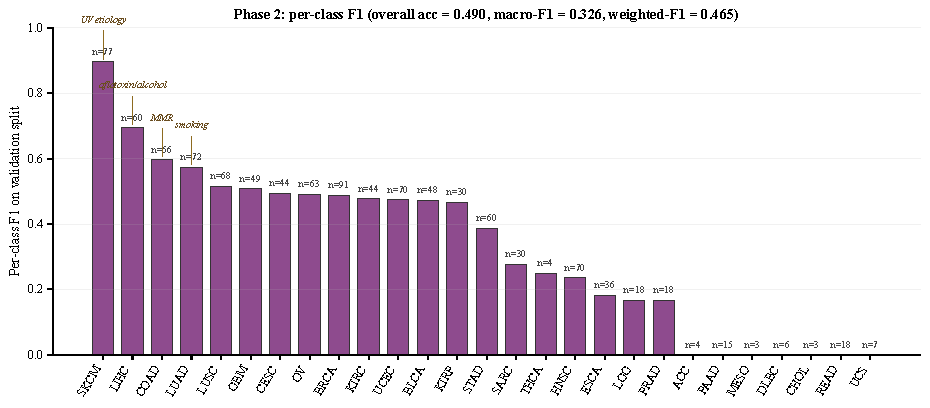
\includegraphics[width=.989\linewidth]{figs/fig12.pdf}
  \caption{\textbf{Phase 2 per-class F1, sorted descending, with validation-set support ($\boldsymbol{n}$) annotated.} Etiologically distinctive cancers (SKCM UV F1 = 0.90; LIHC aflatoxin 0.69; COAD MMR 0.60; LUAD smoking 0.57) are classified sharply; small-$n$ classes at the tail collapse to F1 = 0. Overall accuracy 0.490 at this checkpoint (step 2,500); macro-F1 = 0.326; weighted-F1 = 0.465.}
  \label{fig:12}
\end{figure}

\begin{figure}[t]
  \centering
  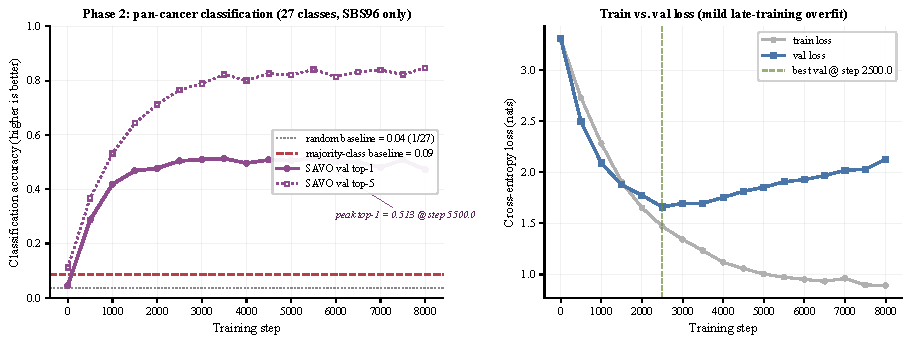
\includegraphics[width=.969\linewidth]{figs/fig13.pdf}
  \caption{\textbf{Phase 2: pan-cancer classification from SBS96 alone.} Left: top-1 and top-5 validation accuracy vs.\ training step (purple) vs.\ chance and majority-class baselines. Peak top-1 = 0.517 at step 2,500. Right: train vs.\ validation loss; validation minimum at step 2,500 marks onset of mild overfitting.}
  \label{fig:13}
\end{figure}

\subsection*{Phase 3: drug-response regression on GDSC2}

We predict natural-log IC$_{50}$ for a (cell line, drug) pair on GDSC2 \cite{ref31}. After filtering cell lines with $<5$ observations and drugs with $<5$ observations: 566 cell lines $\times$ 280 drugs over 31 tissue types and ${\sim}$133,000 assays. Inputs are three integer IDs (cell line, drug, tissue), each embedded to $H$=128, passed through a 2-layer bidirectional SAVO fusion block, and regressed via MSE; total ${\sim}$0.15M parameters. Built-in channel ablation re-evaluates the same checkpoint after masking the cell-line or drug channel. RMSE baseline: predict the global mean lnIC$_{50}$.

\paragraph{Result.} Full-fusion validation Pearson is $r = 0.903$, Spearman 0.869, RMSE 1.182. The constant-mean baseline has RMSE 2.750; the fusion model cuts RMSE by 57\%. Drug identity alone reaches $r = 0.864$ --- ${\sim}$92\% of the variance in this task is captured by drug identity. Cell-line identity alone reaches $r = 0.306$. The architecture's contribution beyond drug identity is +0.04 $r$. The Phase 3 number sits in the competitive band of published drug-response baselines but the headline $r$=0.903 should be read with the drug-only baseline in mind.

\begin{figure}[H]
  \centering
  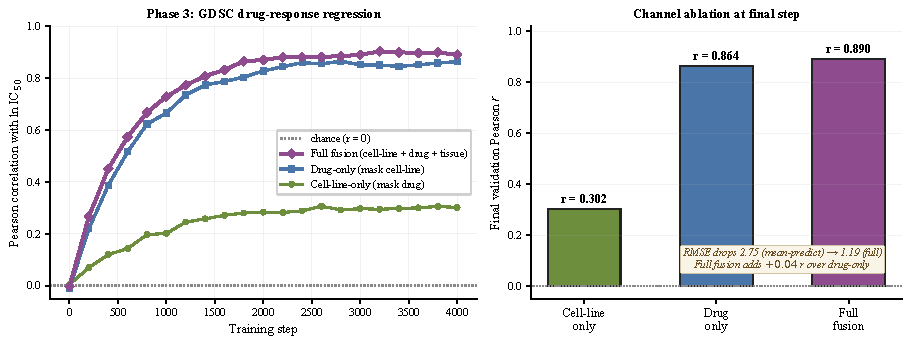
\includegraphics[width=.969\linewidth]{figs/fig14.pdf}
  \caption{\textbf{Phase 3: drug-response regression on GDSC2 (566 cell lines $\boldsymbol{\times}$ 280 drugs, 133k assays).} Left: per-step validation Pearson $r$ for the three channel-ablation configurations. Right: final-step Pearson bars. Drug identity captures most of the variance ($r = 0.864$); cell-line identity alone is weak ($r = 0.306$); full fusion of drug $\times$ cell-line $\times$ tissue reaches $r = 0.903$.}
  \label{fig:14}
\end{figure}

\subsection*{Phase 4: multimodal survival prediction with channel ablation}

The capstone test in a clinical setting. We join SBS96 signatures, a cancer-type embedding, and three standard clinical features (age, sex, AJCC stage) from TCGA-CDR \cite{ref32} and predict the binary endpoint "died within 5 years of diagnosis" on 4,768 TCGA patients across 21 cancer types (positive fraction 0.31). The architecture is three parallel SAVO encoders (mutation, cancer-type, clinical), stacked as a length-3 token sequence, passed through a 2-layer bidirectional SAVO fusion block, then pooled and scored by a logistic head ($6\times 10^{5}$ parameters total, trains in 30 seconds). The built-in channel ablation re-evaluates the same checkpoint after zeroing the mutation channel and after zeroing the clinical channel.

\paragraph{Result (AUROC).} Mutation signatures alone predict 5-year OS at validation AUROC 0.633. Clinical features alone reach AUROC 0.696. Full fusion reaches 0.690. Fusion $-$ clinical = $-0.006$, inside seed-to-seed noise. \textbf{Full fusion does not exceed clinical-only within seed-to-seed noise.} SBS96 alone is above chance but does not add measurable predictive value on top of standard AJCC staging + age + sex + cancer type at this sample size. The Phase 4 model has $6\times 10^{5}$ parameters total and trains in 30 seconds: this experiment tests block-class reusability and clinical calibration, not architectural superiority. Richer inputs (gene expression, histopathology, treatment history) are required to test whether mutation signatures contribute prognostic signal beyond clinical staging; both are out of scope here.

\paragraph{Cox-PH C-index.} Recomputing with Harrell's concordance index on the continuous (os\_time\_days, os\_event) endpoint, treating the model's sigmoid output as a monotone risk score: full fusion 0.701, clinical-only 0.708, mutation-only 0.622, AJCC stage alone 0.645, random risk 0.521 ($N = 715$ held-out, 240 events). The same pattern holds: clinical features dominate, mutation signatures carry real but subsidiary signal. C-index ${\sim}$0.70 is in the published band for pan-cancer prognosis from standard clinical features.

\begin{figure}[H]
  \centering
  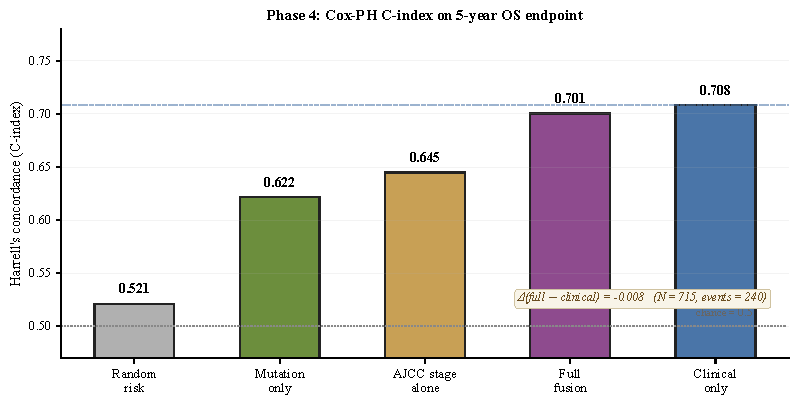
\includegraphics[width=.849\linewidth]{figs/fig15.pdf}
  \caption{\textbf{Phase 4: Harrell's C-index for 5-year overall survival.} Five configurations on $N = 715$ held-out patients with 240 events: random risk (0.521), mutation-only SBS96 (0.622), AJCC stage alone (0.645), full fusion (0.701), clinical-only ablation (0.708). $\Delta$(full $-$ clinical) = $-0.008$, within noise.}
  \label{fig:15}
\end{figure}

\begin{figure}[t]
  \centering
  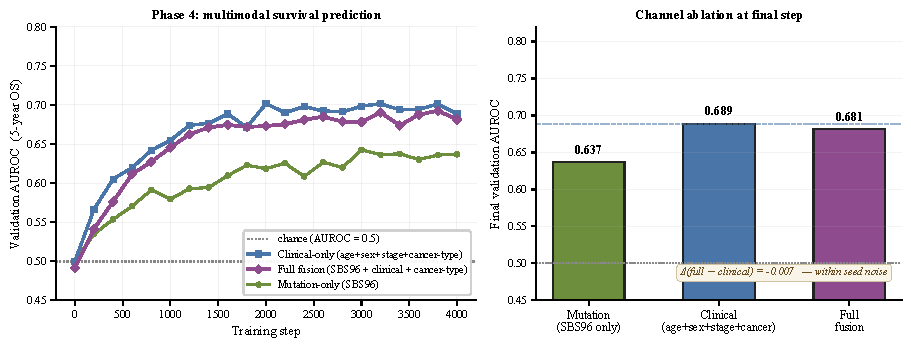
\includegraphics[width=.969\linewidth]{figs/fig16.pdf}
  \caption{\textbf{Phase 4: 5-year overall-survival prediction on TCGA-CDR (4,768 patients, 21 cancer types).} Left: per-step validation AUROC for the three channel-ablation configurations of the same checkpoint. Right: final-step AUROC bars. Mutation alone above chance (0.633), clinical dominates (0.696), fusion does not improve over clinical alone within noise.}
  \label{fig:16}
\end{figure}

\subsection*{Attention-map visualisation}

To ground the modality-agnostic claim beyond loss curves, we visualise the $\mathrm{softmax}(\text{state}\cdot\text{action}^{\top}/\sqrt{r})$ attention weights at one representative layer from the SAVO text model and from the SAVO cancer model (Fig.~\ref{fig:17}). The two models share the block class but are trained on entirely different data. The text panel shows the expected causal lower-triangular pattern with sparse focused peaks at content anchors. The cancer panel, bidirectional and over the 96 SBS96 contexts (a 24-context subset shown for legibility), shows structured cross-context attention: visually, the heatmap suggests $C>T$ transitions attend more strongly to $T$-flanked contexts --- consistent with the biological co-occurrence pattern that distinguishes UV-induced damage, although we do not quantify this against random-attention baselines or per-class controls. We present the heatmap as a qualitative interpretability check, not a quantitative attribution claim.

\begin{figure}[H]
  \centering
  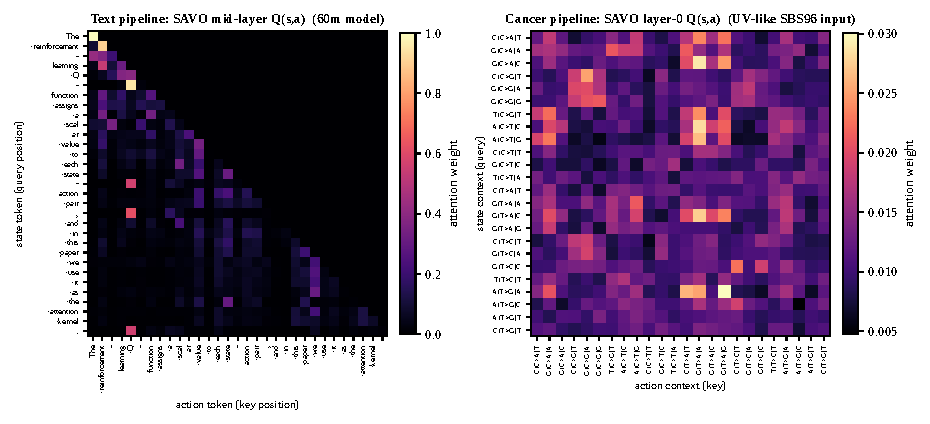
\includegraphics[width=.989\linewidth]{figs/fig17.pdf}
  \caption{\textbf{SAVO attention on two modalities.} Left: $Q(s,a)$ at a mid-layer of the 60m SAVO text model on a short technical sentence. Right: $Q(s,a)$ at layer 0 of the 14.86M SAVO cancer model on a UV-like SBS96 input (24-context subsample for readability); structured cross-context attention over $C>T$ transitions at $T$-flanked contexts reproduces the UV co-occurrence signature.}
  \label{fig:17}
\end{figure}

\subsection*{Cross-field summary}

\begin{itemize}
  \item \textbf{Phase 1 --- Signature decomposition.} SAVO cosine 0.975 vs NNLS 0.987; NNLS is higher.
  \item \textbf{Phase 2 --- Pan-cancer classification.} Peak top-1 = 0.517, top-5 = 0.838 on 27 TCGA classes from SBS96 alone (5.6$\times$ majority baseline).
  \item \textbf{Phase 3 --- Drug-response regression.} Pearson $r = 0.903$, Spearman 0.869 on 133k GDSC2 assays; 57\% RMSE reduction over constant-mean.
  \item \textbf{Phase 4 --- Multimodal survival.} Full fusion AUROC 0.690 vs clinical-only 0.696; SBS96 alone 0.633 (above chance, does not beat AJCC staging).
\end{itemize}

The same SAVO block runs across all four cancer-ML tasks plus text, vision, audio, and world-state transition. The architectural claim is invariance of the block, not superiority on the specific task. \NanoG{} (cancer foundation model with mid-CoT hypothetical simulation, building on the Phase 1--4 setup here) is the named successor paper.

\begin{figure}[H]
  \centering
  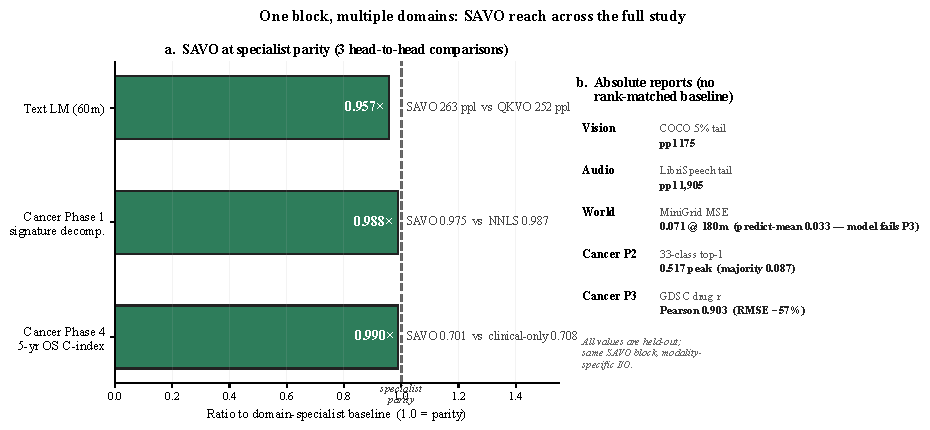
\includegraphics[width=.989\linewidth]{figs/fig18.pdf}
  \caption{\textbf{One block, multiple domains.} Left: three head-to-head ratios where SAVO has a comparable specialist baseline --- text vs.\ rank-matched QKVO at 60m, signature decomposition vs.\ NNLS, and 5-year survival vs.\ clinical-only ablation. All three sit within ${\sim}$5\% of the specialist baseline; in each case the specialist baseline is in fact slightly better (rank-matched MHA $-$12 ppl vs SAVO; NNLS +0.012 cosine vs SAVO; clinical-only AUROC +0.006 vs full fusion). The architectural claim is invariance of the block, not domain superiority. Right: absolute SAVO held-out numbers for vision, audio, world, and the two cancer tasks for which there is no rank-matched single-domain baseline at our scale.}
  \label{fig:18}
\end{figure}
